\section{Microprocessors}

\begin{figure}[H]
    \centering
    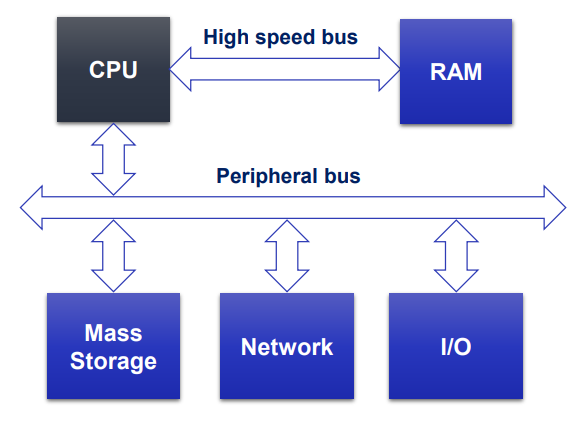
\includegraphics[width=0.75\linewidth]{images/micpro.png}
    \caption{Microprocessor architecture}
\end{figure}
The key features of microprocessor-based applications include:
\begin{itemize}
    \item \textit{Flexibility}: this encompasses maintainability and the ability to evolve the application. 
    \item \textit{Time To Market}: this refers to the duration required to bring a product to the customer.
    \item \textit{Easy upgrade}: software solutions can be updated and improved with minimal disruption.
    \item \textit{Cost}: the overall cost is volume-dependent. 
        Design costs are incurred only once, while production expenses are primarily linked to the cost of silicon.
\end{itemize}
This approach is cost-effective since embedded systems often do not require the full processing power of a microprocessor.

While an equivalent hardware solution may generally provide better performance, microprocessor architectures are optimized for flexibility.  
While software implementations are typically easier to develop than hardware solutions, modifying hardware to meet new requirements is often simpler, with performance advantages remaining on the hardware side.

Designing a software solution necessitates a comprehensive understanding of the microprocessor architectures available in the market. 
The characteristics of the problem (algorithm) should guide the designer, alongside non-functional constraints such as performance, cost, development time, and power consumption. 
The initial step before selecting a specific processor is determining the appropriate class of processor and the form in which it will be acquired.

\subsection{Taxonomy}
Processors can be categorized into two main types:
\begin{itemize}
    \item \textit{Application Specific Processors} (ASP): these processors are tailored for specific classes of applications that require high performance.
    \item \textit{General Purpose Processors} (GPP): these processors are not optimized for any particular application.
\end{itemize}
In typical embedded systems, a multi-processor solution often employs GPPs for supervising and controlling the activities of one or more ASPs.

\paragraph*{Availability}
Processors can further be classified as follows:
\begin{itemize}
    \item \textit{Components Off The Shelf} (COTS): these are standard chips purchased and mounted onto a printed circuit board along with the necessary interfaces to integrate with the rest of the system.
    \item \textit{Intellectual Property} (IP): this involves purchasing the design specifications of a microprocessor. 
        In this case we may classify the microprocessors depending on the description as: soft macro (HDL) or hard macro (layout). 
\end{itemize}

\paragraph*{Selection}
The selection process is based on: 
\begin{itemize}
    \item \textit{Class}: the nature of the algorithm and the operations are the primary drivers.
    \item \textit{Form}: the target architecture of the system. 
    \item \textit{Performance}: a key metric for performance is the average number of Instructions Per Clock (IPC). 
        Million Instructions Per Second (MIPS) serves as an absolute measure of throughput but can be misleading when comparing processors with different Instruction Sets.
        For floating-point operations, MFLOPS is commonly used, while specialized architectures like Digital Signal Processors (DSPs) often use Million Multiply Accumulate operations Per Second (MMACS), and Network Processor (NP) typically measure the average number of processed packets per time unit.
    \item \textit{Power}: both average power and peak power are important metrics for estimating the maximum or average power consumption of the overall system. 
        A combined measure of power and speed is often used.
\end{itemize}
Other important considerations include:
\begin{itemize}
    \item \textit{Memory}: the bandwidth and size requirements of the application can impose hard constraints. 
        In some cases, only internal memory may be available, making external memory utilization impractical. 
    \item \textit{Peripherals}: embedded systems often process external signals and control physical devices. 
        Designers can either choose an architecture focused on computation and design the rest of the system accordingly or opt for a single-chip solution that integrates computing, interfacing, and peripherals. 
    \item \textit{Software}: he availability of libraries can simplify both the design and validation processes. 
        Differences among SDKs are significant, and factors such as the software compilation flow, code quality, and flexibility offered to the designer are important. 
    \item \textit{Packaging}: packages differs in size, pinout, and materials.
    \item \textit{Certifications}: some certifications are tailored for specific fields, such as MISRA rules for automotive code. 
\end{itemize}

\subsection{General Pupropose Processor}
General Purpose Processors (GPPs) are characterized by a generic architecture that is applicable across a wide range of fields. 
They are commonly found in PCs, and for embedded systems, they are suitable for low-end applications where energy efficiency and performance are not critical, and the application nature is quite heterogeneous.
GPPs handle tasks such as controlling and managing slow interfaces with sensors and enabling interactivity through graphical user interfaces.
The possible architectural styles for GPPs are: 
\begin{itemize}
    \item \textit{Complex Instruction Set Computer} (CISC): allow each arithmetic or logic operation to access data and write results using any available addressing mode. 
        However, in practice, the number of combinations of operations and addressing modes is often limited.
        Despite the complexity, CISC instructions are encoded in variable-length formats, which necessitates more complex fetch and decode units and a higher speed for memory access.
        Some architectures even support vector instructions, enabling operations on multiple registers simultaneously. 
        To enhance throughput, CISC processors often employ intricate pipelining techniques. 
        Additionally, they may alter the order of execution for assembly instructions without changing the program's semantics (out-of-order execution). 
        This complexity makes it difficult for compilers to predict instruction execution status, potentially leading to suboptimal instruction decoding. 
    \item \textit{Reduced Instruction Set Computer} (RISC): utilize a limited number of straightforward instructions. 
        RISC instructions typically have fixed lengths, facilitating balanced pipeline stages and higher clock speeds. 
        RISC employs a load and store architecture for input and output operations. 
        While the limited number of addressing modes can aid performance, effective use of memory hierarchy is crucial for minimizing data access time.
        When comparing RISC and CISC using the same high-level source code, RISC generally requires a higher number of instructions. 
        RISC architectures do not have hardware mechanisms to resolve pipeline conflicts, but their predictable execution allows compilers to generate efficient code. 
        Furthermore, RISC architectures typically exhibit lower power consumption due to their inherent simplicity compared to CISC architectures.
    \item \textit{Superscalar}: multiple execution units, enabling the simultaneous execution of more than one instruction per clock cycle. 
        This parallelism enhances throughput but also increases the complexity of control logic. 
        However, a significant portion of the processor's resources is dedicated to implementing complex scheduling mechanisms and maintaining consistency.
    \item \textit{Very Long Instruction Word} (VLIW): these processors support explicit parallelism of RISC instructions. 
        Once fetched from memory, the VLIW word is decoded in parallel, with individual instructions dispatched to various execution units. 
        This fixed structure shifts the complexity of scheduling onto the compiler.
        Power consumption for VLIW architectures falls between that of simpler RISC and superscalar designs. 
    \item \textit{CISC RISC}: combine out-of-order execution with superscalarity while maintaining compatibility with legacy code. 
        This architecture is more costly, but achieves higher performance. 
    \item \textit{CISC VLIW}: aims for high performance while ensuring backward compatibility. 
        CISC instructions are broken down into basic instructions that can be executed by a VLIW core, which is both simple and efficient.
\end{itemize}

\paragraph*{Comparison}
The comparison between GPPs architecture is outlined in the following table: 
\renewcommand*{\arraystretch}{1.25}
\begin{table}[H]
    \centering
    \begin{tabular}{|l|cccc|}
    \hline
    & \textbf{RISC} & \textbf{CISC} & \textbf{Superscalar} & \textbf{VLIW} \\ \hline
    \textit{Instruction set} & simple & complex & complex & simple \\ \hline
    \textit{Addressing modes} & few & many & many & few \\ \hline
    \textit{Instruction size} & fixed & variable & variable & fixed, large \\ \hline
    \textit{Register file} & single & single & single & multiple \\ \hline
    \textit{Number of registers} & high & low & medium & very high \\ \hline
    \textit{Instruction scheduling} & static & dynamic & dynamic & static \\ \hline
    \textit{Conflict management} & static & dynamic & dynamic & static \\ \hline
    \textit{Compiler complexity} & medium & high & low & very high \\ \hline
    \textit{Parallelism} & absent & absent & implicit & explicit \\ \hline
    \textit{Hardware complexity} & low & high & very high & high \\ \hline
    \textit{Pipeline complexity} & low & high & very high & medium \\ \hline
    \textit{Power consumption} & very low & high & very high & high \\ \hline
    \textit{Typical IPC} & $\approx$ 1 & $<$ 1 & $>$ 1 & $\geq$ 1 \\ \hline
    \end{tabular}
\end{table}
\renewcommand*{\arraystretch}{1}

\subsection{Application Specific Processor}
Embedded systems often require high specialization and a limited set of functions, making GPPs less suitable for certain applications. 
To address these specific needs, Application Specific Processors (ASPs) have been developed.
The main ASPs architectures are: 
\begin{itemize}
    \item \textit{Digital Signal Processor} (DSP): microprocessors designed specifically for numerical computing tasks based on the multiply accumulate (MAC) operation: 
        \[z_{t+1} = z_t + x \cdot y\]
        To achieve high efficiency, DSPs are designed to optimize the execution of loops. 
        This is possible due to certain characteristics of loop structures, such as having small bodies—typically around ten assembly instructions—where the control loop variable remains unchanged.
        To combat this, DSP architectures often include high-bandwidth interfaces and sophisticated memory hierarchies for enhanced memory access speed. 
        Many modern ASPs processors are based on VLIW architectures to optimize performance. 
    \item \textit{Network processor} (NP): specialized microprocessors tailored for processing network packets, which use high levels of parallelism to handle the demands of network applications.
        Designing an NP can be quite complex due to the ever-evolving networking functionalities and protocols. 
        To maximize performance, NPs incorporate dedicated hardware for high-speed I/O interfaces, queue management, cryptographic cores, and multiple RISC cores (for supervision and management).
        In some cases we may have specialized NP called Packet Processors (PPs) or Channel Processors (CPs) to manage multiple independent data channels. 
    \item \textit{Microcontrollers}: these devices integrate peripherals and interfaces onto a single chip, making them ideal for applications that do not demand high computational power but do require careful management of hardware resources and development time. 
        The lack of memory interfaces can increase pin counts, prompting some architectures to employ multiplexing techniques to limit this increase. 
        Microcontrollers typically provide a variety of peripheral interfaces. 
        The SDKs available for microcontrollers can vary significantly, ranging from basic C compilers to comprehensive frameworks that assist in performance analysis and configuration management.
\end{itemize}